\documentclass{report}

\usepackage{verbatim}
\usepackage{graphicx}
\usepackage{hyperref}
\usepackage{float}

\begin{document}

\chapter*{User Documentation}

\section*{Running the program}
To compile and run the software, you need to have \texttt{dotnet} and \texttt{npm} available on your system.
The required .NET Runtime version is 8.X.

Compilation can be done using these commands (run in the root directory of the project):
\begin{verbatim}
dotnet tool install fable
dotnet tool restore
dotnet restore
npm update
npm run build
\end{verbatim}

The webpage is then available in the \texttt{dist} directory. It can be run by using the command:
\begin{verbatim}
npm run server
\end{verbatim}
This will open a local HTTP server on \url{http://127.0.0.1:5173/} which hosts the software.

\section*{Using the software}

\begin{figure}[H]
    \centering
    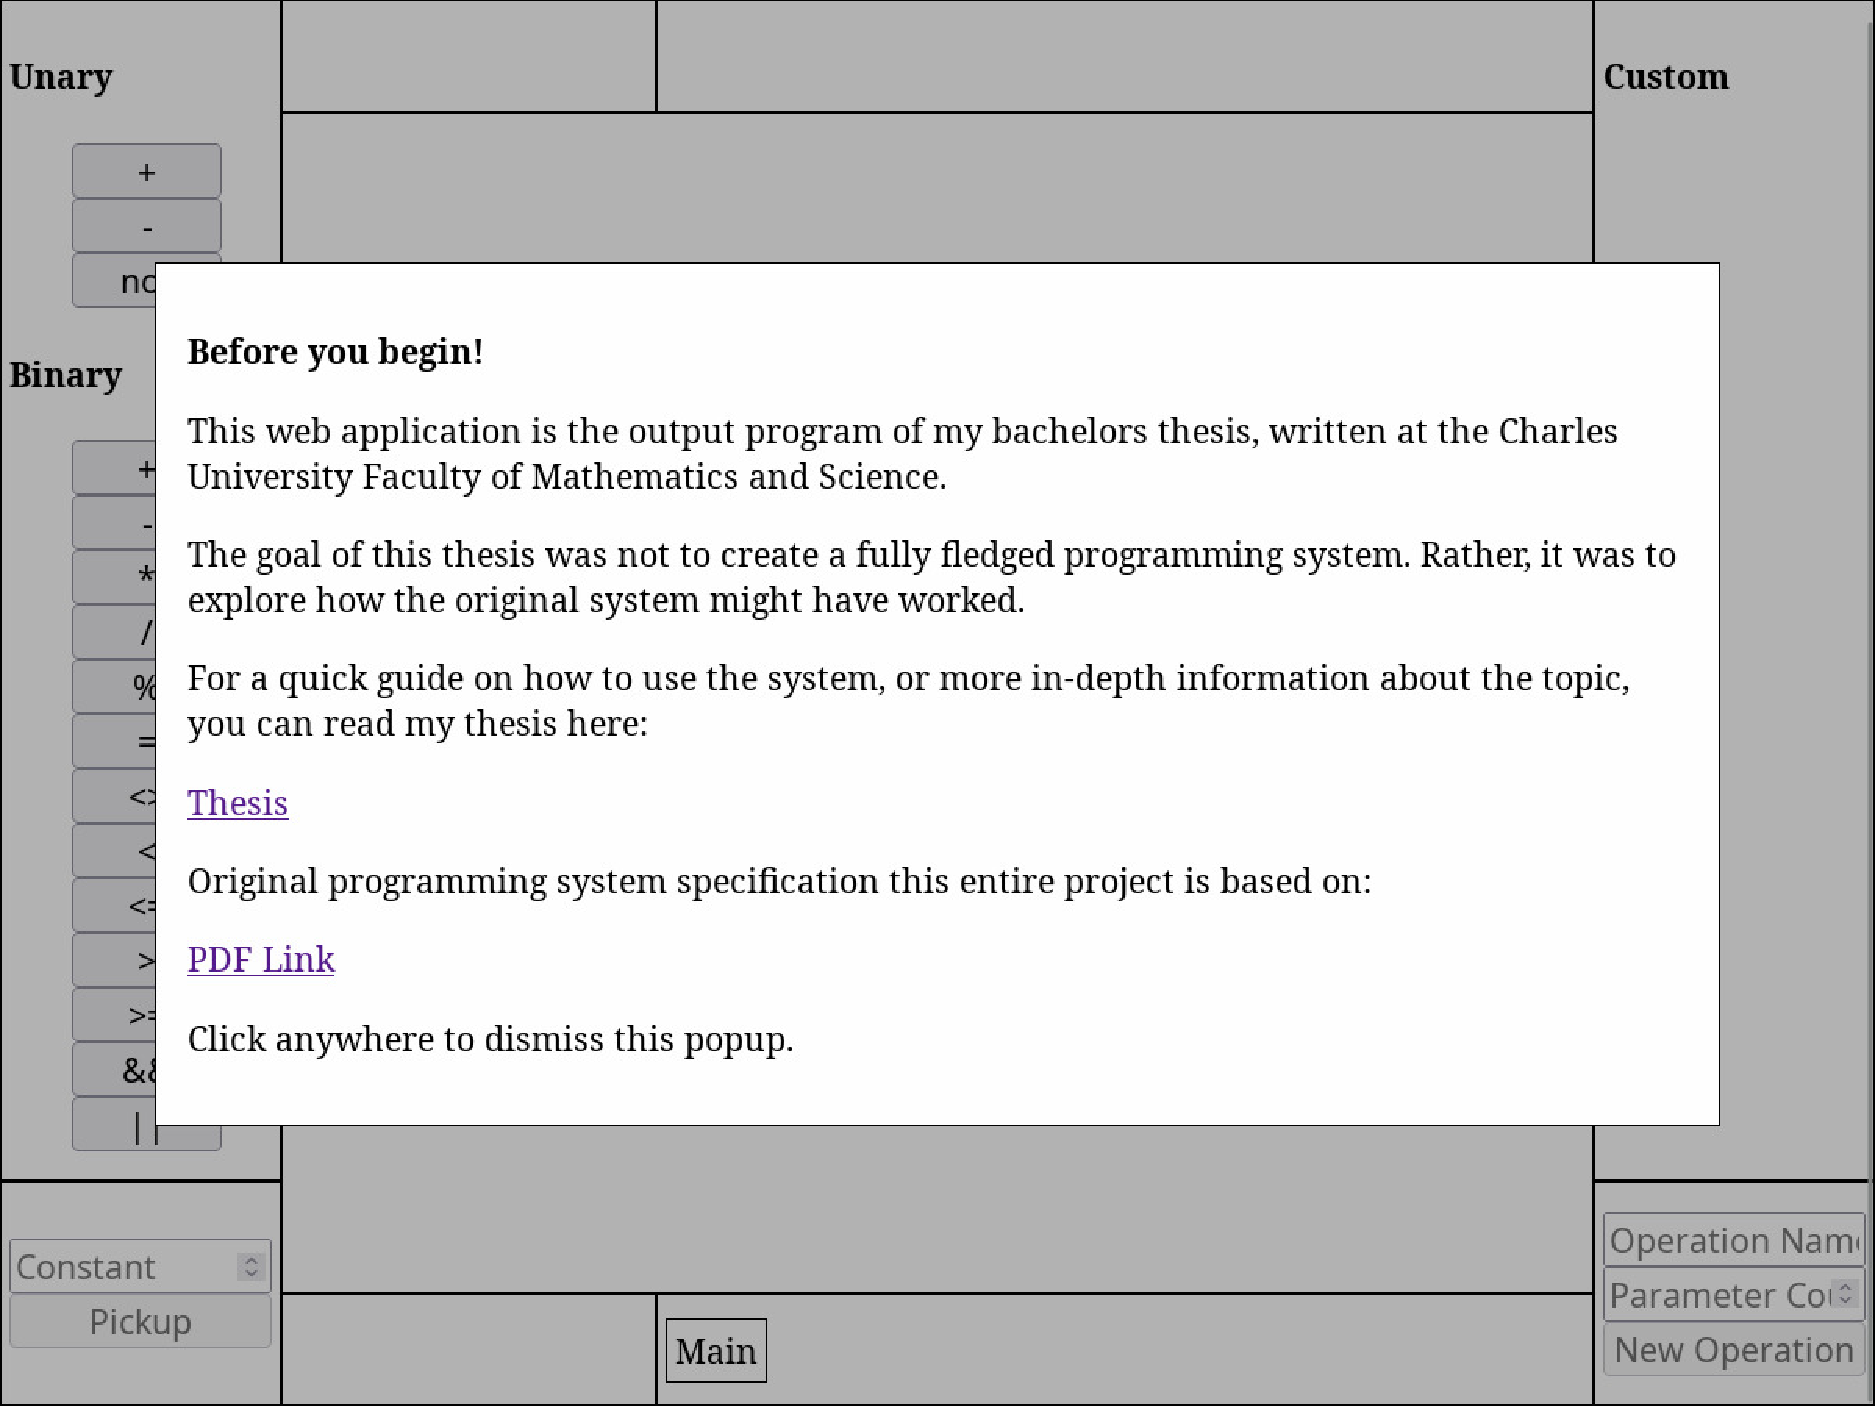
\includegraphics[width=1\textwidth]{img/app_intro.pdf}
    \caption{The first screen the user sees}
    \label{fig:intro}
\end{figure}

The software is a web application that can be accessed through a web browser. The first thing the user sees is an intro popup. It can be dismissed by clicking anywhere on the screen.

\begin{figure}[H]
    \centering
    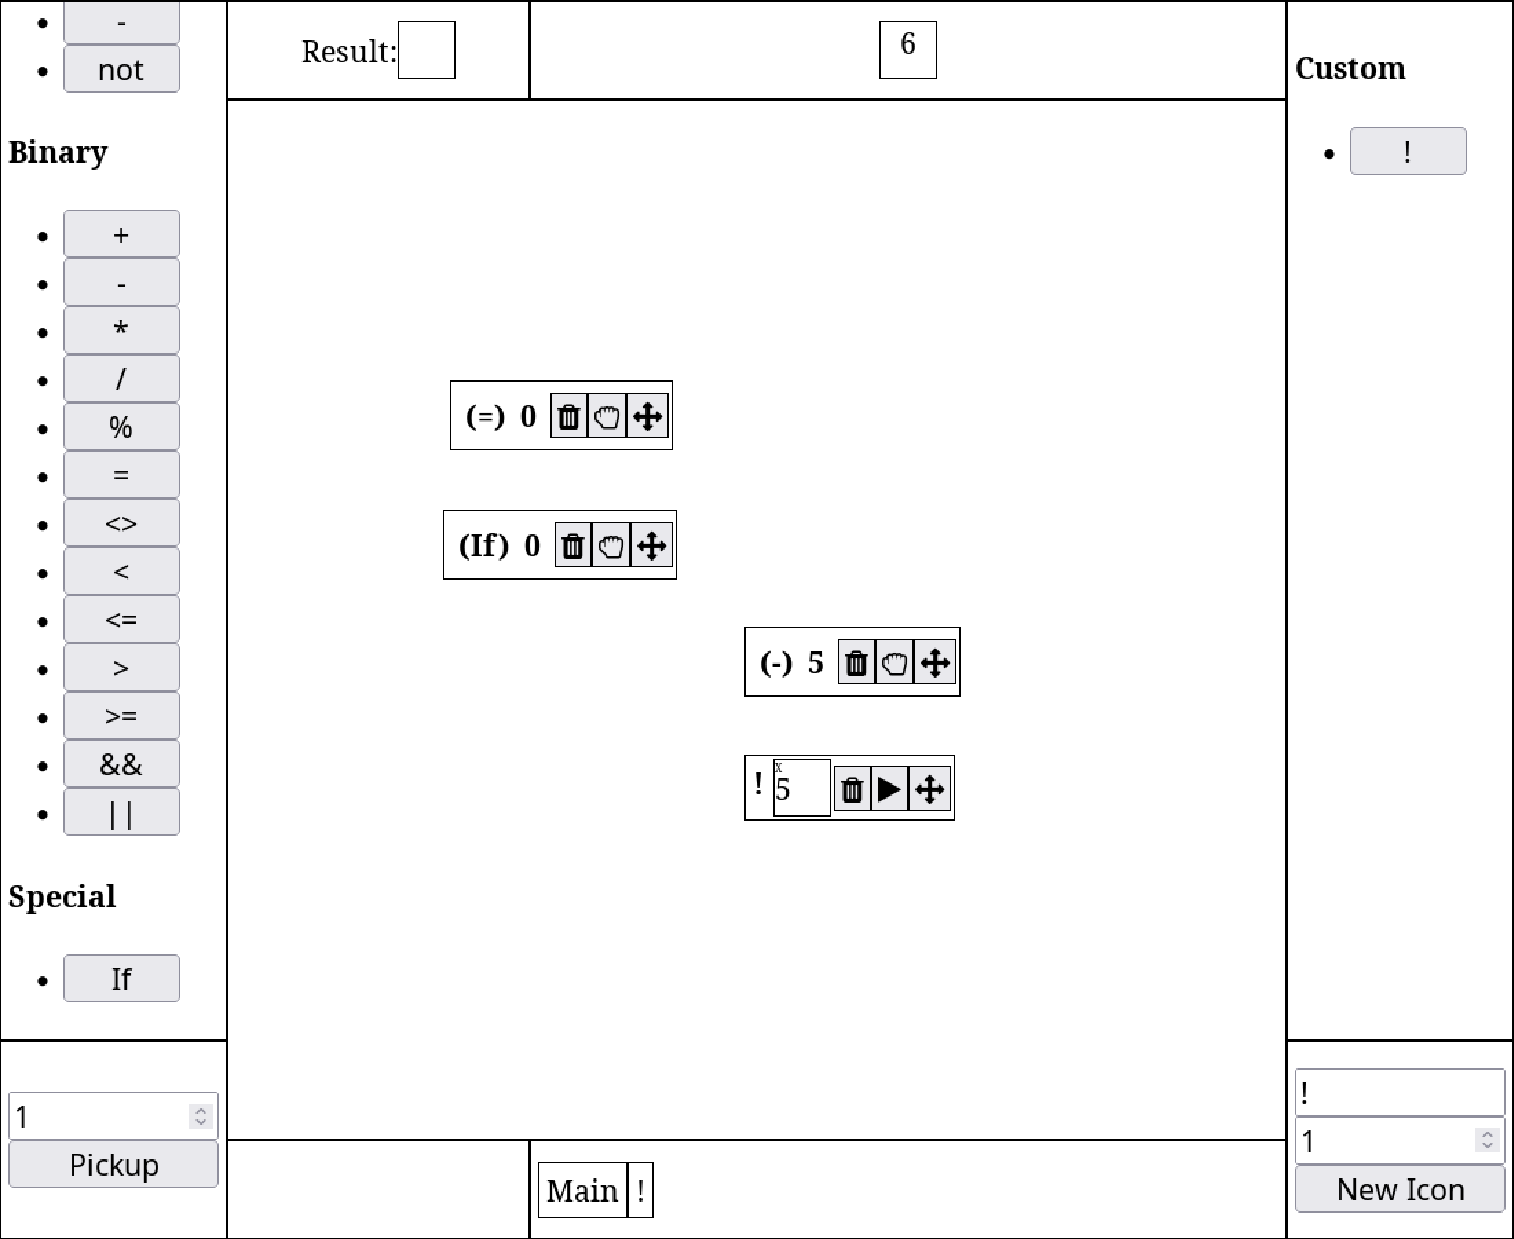
\includegraphics[width=1\textwidth]{img/app.pdf}
    \caption{The GUI of the software}
    \label{fig:gui}
\end{figure}

\noindent
The GUI is split into nine parts. The split parts can be seen in figure \ref{fig:gui}.
The most common interaction that the user will perform is picking up objects and placing them down.
An object is picked up by clicking on it, and placed by clicking on the target.
The user can pickup three types of objects. A number, a new icon, and an existing icon.
The currently picked up object is displayed in the bottom middle left of the screen.
In the example, nothing is being held.

\subsubsection{Numbers}
A number can be picked up from various sources.
The first source is the \emph{constant spawner}, which is the input field and corresponding button in the bottom left of the GUI.
The user can write a number into the input field (a 1 is written in the example), and then click the button to spawn the number.
The button can be clicked only when the input field contains a valid number.

Numbers can also be picked up from the top middle right of the GUI. This area contains the parameters of the current custom operation.
In the example, the area only contains a 6. Clicking on it will pick up the number.

The last source of numbers are icons. We can pick up the result from an icon by clicking on the closed hand button.
This is the middle button in the bottom list of every icon. This icon is only present if an icon is evaluated.
In other words, a number can only be picked up from an icon if it has a result.

Numbers can be placed in two places. The first is any parameter box of an icon. A parameter box that contains 5 can be seen in the example, in the bottom-right-most icon with the \texttt{!} symbol.
The second valid target for a number is the \texttt{Result} box in the top middle left of the screen.

\subsubsection{New Icons}
The user can also pick up new icons. New icons are spawned by clicking on a button in one of the \emph{icon spawners} on the screen.
These are the lists located on the left and right of the screen. The left icon spawner contains pre-defined icons, and the right one contain custom ones.
When one of these buttons are clicked, a new icon of the corresponding type becomes the held object.

The only valid target for icons is the icon canvas. This is the rectangular area in the middle of the screen. In the example, it already contains four icons.
We can place the new icon by clicking on any free space in the canvas. This creates a new icon with the specified type.

\subsubsection{Existing Icons}
Icons have three parts. The first is the name of the operation that the icon performs when evaluated. In our example, we can see the \texttt{=}, \texttt{If}, \texttt{-} and \texttt{!} icons.

The second part serves two purposes.
If an icon is not evaluated, this part holds parameter boxes. We can see a parameter box in the bottom-right-most icon. This parameter box contains a 5.
All parameter also have a small \texttt{X} button in the top left of their rectangle. This button can be clicked to clear the respective parameter box.
Icons have a parameter box for every parameter that the operation requires. The \texttt{!} icon requires one parameter, and the \texttt{-} icon requires two.
If an icon is evaluated, then the parameter boxes are replaced by the result of the operation. We can see the result of the \texttt{-} icon in the middle-right icon, which is 5.
Evaluated icons also have their name surrounded by parantheses in bold text, to differentiate them from unevaluated icons.

The third part of the icon contains three buttons.
The first button with the trash can icon deletes the icon. This button is present on every icon.
The second button changes depending on if the icon is evaluated or not.
If it is not evaluated, then this button evaluates the icon. Evaluation of an icon means that the underlying operation that the icon was created with is performed.
This requires all parameters of the icon to be present. If they are not, pressing the button does nothing.
When an icon is evaulated, this button changes to a closed fist button, which picks up the result as a number when clicked.
The last button is a move button. It allows the user to move the icon elsewhere on the canvas. Similarly to creating new icons,
the only valid target for placing an existing icon is an empty spot on the icon canvas.

\subsubsection{Custom operations}
A new custom operation can be created using the input fields with their corresponding button on the bottom right of the screen.
The first input field is for specifying the name of the custom operation, and the second one is for specifying the number of parameters that the operation requires.
When these input fields have valid inputs, the button can be clicked to create a new custom operation. Creating a new custom operation places it in the right icon spawner.

\subsubsection{Tabs}
In the bottom middle right of the screen, we have a tab view. This view shows the call stack of tabs, which can be understood as instances of custom operation evaluation.
The \texttt{Main} tab is always present. The rightmost tab is the one that we are currently seeing. The only way to close a tab is to place a number in the result box.
Opening a tab can only be done by hitting a trap in a custom operation.

\subsubsection{Evaluation}
The main purpose of the program is creating custom operation using programming by demonstration on concrete data.
This means that most actions that the user performs are saved somewhere within the custom operation to be used later.
The only way a user can finish such a list of actions is by placing a number in the result box.
This closes the topmost tab, and starts evaluating the previous one.
If this evaluation also ends with the action of saving a result, then that tab closes too.
This happens again and again until we either hit a trap or end up in the \texttt{Main} tab.

Another important concept for evaluation are traps. These are the only other possible way of ending an action list.
When a trap is encountered during evaluation, a new tab is opened and the state that caused the trap is shown.
We are then prompted to define the next operations that should be performed on this state.
We can hit another trap in this new tab, which opens another tab, and so on.

\end{document}